\documentclass[border=16pt]{standalone}
\usepackage{tikz}
\usetikzlibrary{shapes,arrows.meta,positioning,calc}
\renewcommand{\familydefault}{\sfdefault}

\begin{document}
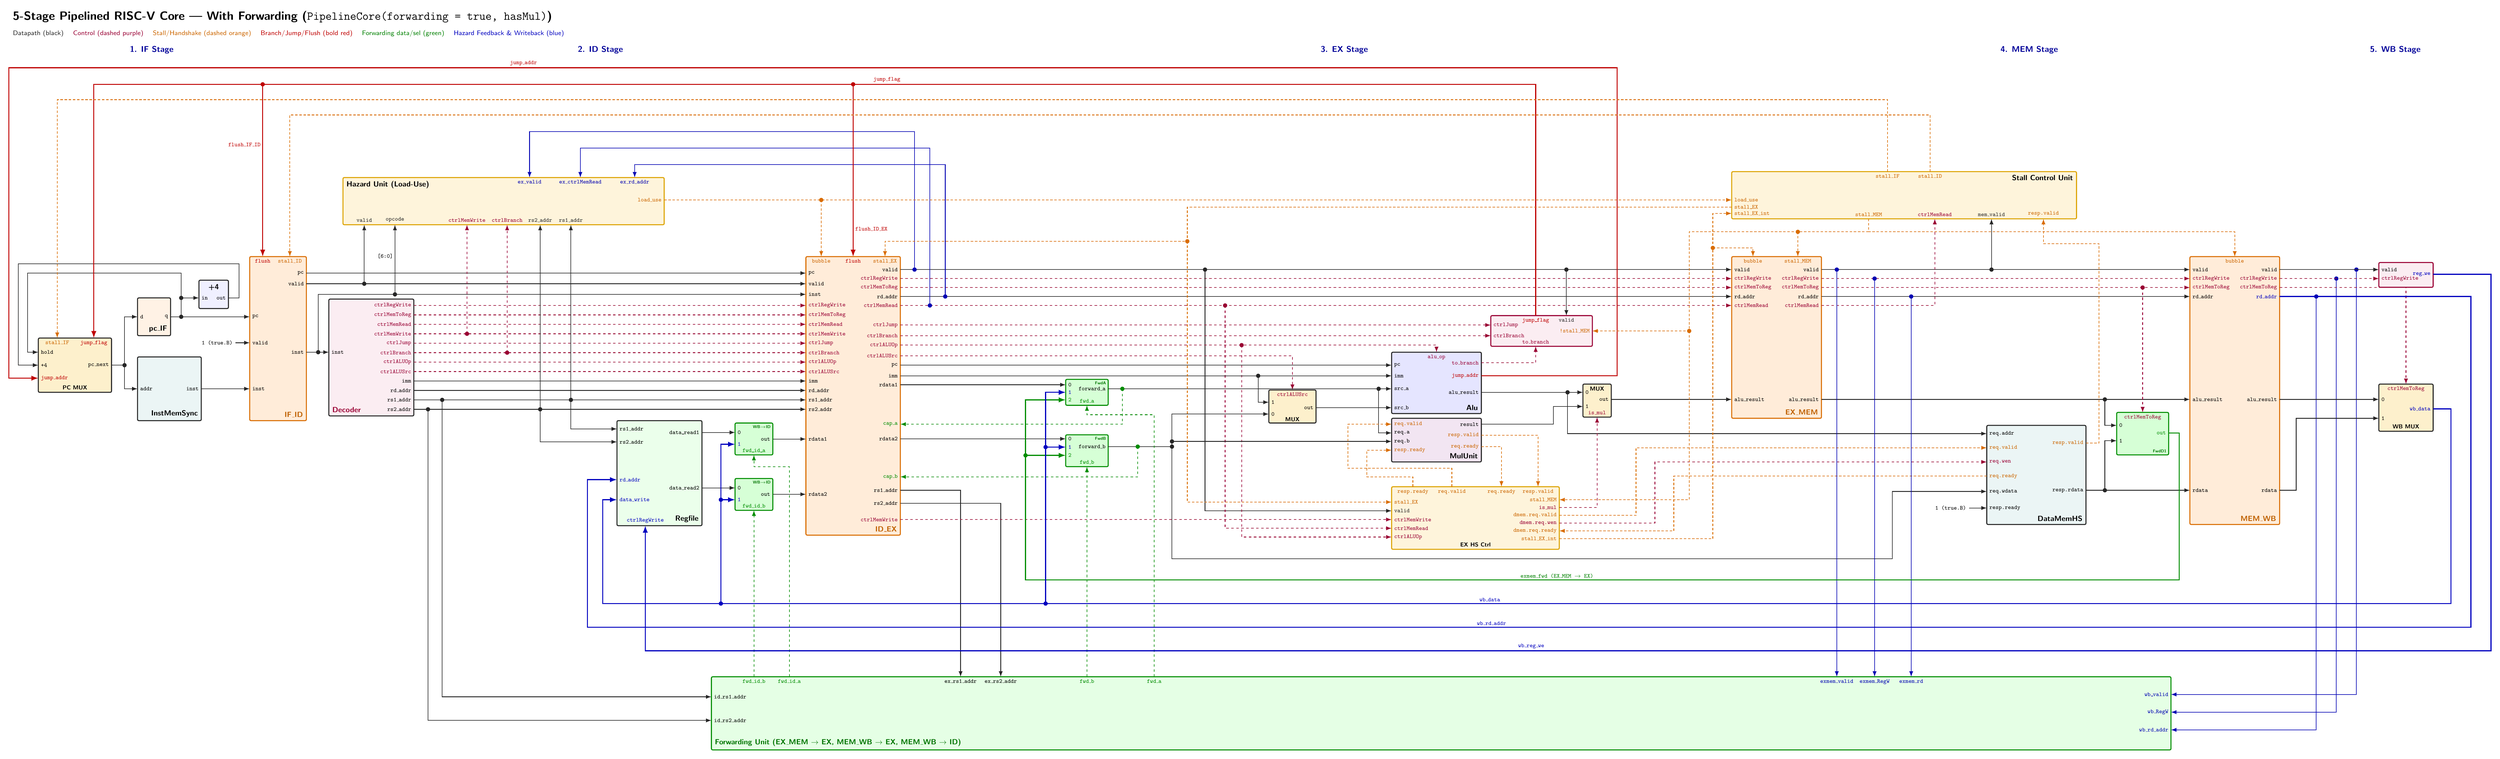
\begin{tikzpicture}[
    >=Latex,
    font=\scriptsize,
    box/.style={draw=black!85, very thick, fill=white, rounded corners=1.5pt},
    preg/.style={draw=orange!85!black, very thick, fill=orange!15, rounded corners=1.5pt},
    hbox/.style={draw=amber!90!black, very thick, fill=amber!14, rounded corners=1.5pt},
    fbox/.style={draw=green!55!black, very thick, fill=green!10, rounded corners=1.5pt},
    pinL/.style={anchor=west, font=\scriptsize\ttfamily, inner sep=3pt},
    pinR/.style={anchor=east, font=\scriptsize\ttfamily, inner sep=3pt},
    pinT/.style={anchor=north, font=\scriptsize\ttfamily, inner sep=3pt},
    pinB/.style={anchor=south, font=\scriptsize\ttfamily, inner sep=3pt},
    modtitle/.style={anchor=south east, font=\small\bfseries, inner sep=4pt},
    wire/.style={->, thick, draw=black!85},
    bwire/.style={->, very thick, draw=red!75!black},
    cwire/.style={->, thick, draw=purple!80!black, dashed},
    swire/.style={->, thick, draw=orange!85!black, densely dashed},
    fwire/.style={->, very thick, draw=green!55!black},
    fcwire/.style={->, thick, draw=green!55!black, dashed},
    fbwire/.style={->, thick, draw=blue!70!black},
    wbwire/.style={->, very thick, draw=blue!75!black},
    lbl/.style={font=\scriptsize\ttfamily, inner sep=2pt},
    dot/.style={circle, fill=black!85, inner sep=1.8pt}
]
\definecolor{amber}{RGB}{245,180,0}

% =========================================================================
% Title, Legend & Stage Headers
% =========================================================================
\node[font=\Large\bfseries, anchor=west] at (-4.5, 16.00) {5-Stage Pipelined RISC-V Core --- With Forwarding (\texttt{PipelineCore(forwarding = true, hasMul)})};
\node[font=\footnotesize, anchor=west] at (-4.5, 15.30) {\textcolor{black!85}{Datapath (black)} \quad \textcolor{purple!80!black}{Control (dashed purple)} \quad \textcolor{orange!80!black}{Stall/Handshake (dashed orange)} \quad \textcolor{red!75!black}{Branch/Jump/Flush (bold red)} \quad \textcolor{green!50!black}{Forwarding data/sel (green)} \quad \textcolor{blue!75!black}{Hazard Feedback \& Writeback (blue)}};

\node[font=\bfseries\normalsize, text=blue!60!black] at (1.5, 14.60)  {1. IF Stage};
\node[font=\bfseries\normalsize, text=blue!60!black] at (20.5, 14.60) {2. ID Stage};
\node[font=\bfseries\normalsize, text=blue!60!black] at (52.0, 14.60) {3. EX Stage};
\node[font=\bfseries\normalsize, text=blue!60!black] at (81.0, 14.60) {4. MEM Stage};
\node[font=\bfseries\normalsize, text=blue!60!black] at (96.5, 14.60) {5. WB Stage};

% =========================================================================
% TOP CONTROL UNITS: Load-Use Hazard Unit & Stall Control Unit
% =========================================================================
% Load-Use Hazard Unit (x: 9.6 .. 23.2, y: 7.20 .. 9.20) -- 3 SEPARATE ex_* pins!
\draw[hbox] (9.6, 7.20) rectangle (23.2, 9.20);
\node[pinB, text=black!85]        at (10.50, 7.20) {valid};
\node[pinB, text=black!85]        at (11.80, 7.20) {opcode};
\node[pinB, text=purple!80!black] at (14.85, 7.20) {ctrlMemWrite};
\node[pinB, text=purple!80!black] at (16.55, 7.20) {ctrlBranch};
\node[pinB, text=black!85]        at (17.95, 7.20) {rs2\_addr};
\node[pinB, text=black!85]        at (19.25, 7.20) {rs1\_addr};
\node[pinT, text=blue!70!black]   at (17.50, 9.20) {ex\_valid};
\node[pinT, text=blue!70!black]   at (19.65, 9.20) {ex\_ctrlMemRead};
\node[pinT, text=blue!70!black]   at (21.95, 9.20) {ex\_rd\_addr};
\node[pinR, text=orange!80!black] at (23.2, 8.25)  {load\_use};
\node[font=\small\bfseries, anchor=north west, inner sep=4pt] at (9.6, 9.20) {Hazard Unit (Load-Use)};

% Stall Control Unit (x: 68.4 .. 83.0, y: 7.45 .. 9.45 -> spacious 1.60 cm corridor above EX_MEM!)
\draw[hbox] (68.4, 7.45) rectangle (83.0, 9.45);
\node[pinL, text=orange!80!black] at (68.4, 8.25) {load\_use};
\node[pinL, text=orange!80!black] at (68.4, 7.95) {stall\_EX};
\node[pinL, text=orange!80!black] at (68.4, 7.68) {stall\_EX\_int};
\node[pinT, text=orange!80!black] at (75.0, 9.45) {stall\_IF};
\node[pinT, text=orange!80!black] at (76.8, 9.45) {stall\_ID};
\node[pinB, text=orange!80!black] at (74.2, 7.45) {stall\_MEM};
\node[pinB, text=purple!80!black] at (77.0, 7.45) {ctrlMemRead};
\node[pinB, text=black!85]        at (79.4, 7.45) {mem\_valid};
\node[pinB, text=orange!80!black] at (81.6, 7.45) {resp.valid};
\node[font=\small\bfseries, anchor=north east, inner sep=4pt] at (83.0, 9.45) {Stall Control Unit};

% =========================================================================
% 1. IF STAGE
% =========================================================================
\draw[box, fill=amber!20] (-3.3, 0.1) rectangle (-0.2, 2.4);
\node[pinT, text=orange!80!black] at (-2.50, 2.4) {stall\_IF};
\node[pinT, text=red!75!black]    at (-0.95, 2.4) {jump\_flag};
\node[pinL]                       at (-3.3, 1.80) {hold};
\node[pinL]                       at (-3.3, 1.25) {+4};
\node[pinL, text=red!75!black]    at (-3.3, 0.70) {jump\_addr};
\node[pinR]                       at (-0.2, 1.25) {pc\_next};
\node[font=\scriptsize\bfseries]  at (-1.75, 0.30) {PC MUX};

\draw[box, fill=orange!10] (0.9, 2.5) rectangle (2.3, 4.1);
\node[pinL] at (0.9, 3.30) {d};
\node[pinR] at (2.3, 3.30) {q};
\node[modtitle] at (2.3, 2.5) {pc\_IF};

\draw[box, fill=blue!6] (3.50, 3.65) rectangle (4.75, 4.85);
\node[pinL] at (3.50, 4.10) {in};
\node[pinR] at (4.75, 4.10) {out};
\node[font=\small\bfseries] at (4.125, 4.55) {+4};

\draw[box, fill=teal!8] (0.9, -1.1) rectangle (3.6, 1.6);
\node[pinL] at (0.9, 0.25) {addr};
\node[pinR] at (3.6, 0.25) {inst};
\node[modtitle] at (3.6, -1.1) {InstMemSync};

\draw[preg] (5.65, -1.1) rectangle (8.05, 5.85);
\node[pinT, text=red!75!black]    at (6.20, 5.85) {flush};
\node[pinT, text=orange!80!black] at (7.35, 5.85) {stall\_ID};
\node[pinL] at (5.65, 3.30) {pc};
\node[pinL] at (5.65, 2.20) {valid};
\node[pinL] at (5.65, 0.25) {inst};
\node[pinR] at (8.05, 5.15) {pc};
\node[pinR] at (8.05, 4.70) {valid};
\node[pinR] at (8.05, 1.80) {inst};
\node[modtitle, text=orange!75!black] at (8.05, -1.1) {IF\_ID};

\node[font=\scriptsize, anchor=east] at (5.05, 2.20) {\texttt{1 (true.B)}};
\draw[wire] (5.05, 2.20) -- (5.65, 2.20);

% =========================================================================
% 2. ID STAGE
% =========================================================================
\draw[box, fill=purple!7] (9.0, -0.90) rectangle (12.6, 4.05);
\node[pinL] at (9.0, 1.80) {inst};
\node[pinR, text=purple!80!black] at (12.6, 3.78) {ctrlRegWrite};
\node[pinR, text=purple!80!black] at (12.6, 3.38) {ctrlMemToReg};
\node[pinR, text=purple!80!black] at (12.6, 2.98) {ctrlMemRead};
\node[pinR, text=purple!80!black] at (12.6, 2.58) {ctrlMemWrite};
\node[pinR, text=purple!80!black] at (12.6, 2.18) {ctrlJump};
\node[pinR, text=purple!80!black] at (12.6, 1.78) {ctrlBranch};
\node[pinR, text=purple!80!black] at (12.6, 1.38) {ctrlALUOp};
\node[pinR, text=purple!80!black] at (12.6, 0.98) {ctrlALUSrc};
\node[pinR]                       at (12.6, 0.58) {imm};
\node[pinR]                       at (12.6, 0.18) {rd\_addr};
\node[pinR]                       at (12.6,-0.22) {rs1\_addr};
\node[pinR]                       at (12.6,-0.62) {rs2\_addr};
\node[modtitle, anchor=south west, text=purple!80!black] at (9.0, -0.90) {Decoder};

\draw[box, fill=green!8] (21.2, -5.55) rectangle (24.8, -1.10);
\node[pinL] at (21.2, -1.45) {rs1\_addr};
\node[pinL] at (21.2, -2.00) {rs2\_addr};
\node[pinL, text=blue!75!black] at (21.2, -3.60) {rd\_addr};
\node[pinL, text=blue!75!black] at (21.2, -4.45) {data\_write};
\node[pinB, text=blue!75!black] at (22.4, -5.55) {ctrlRegWrite};
\node[pinR] at (24.8, -1.60) {data\_read1};
\node[pinR] at (24.8, -3.95) {data\_read2};
\node[modtitle] at (24.8, -5.55) {Regfile};

% WB->ID MUX A (x: 26.2 .. 27.8, y: -2.55 .. -1.20)
\draw[box, fill=green!16, draw=green!55!black] (26.2, -2.55) rectangle (27.8, -1.20);
\node[font=\tiny\bfseries, text=green!45!black, anchor=north east, inner sep=2.5pt] at (27.8, -1.20) {WB$\to$ID};
\node[pinL] at (26.2, -1.60) {0};
\node[pinL, text=blue!75!black] at (26.2, -2.10) {1};
\node[pinB, text=green!55!black] at (27.00, -2.55) {fwd\_id\_a};
\node[pinR] at (27.8, -1.88) {out};

% WB->ID MUX B (x: 26.2 .. 27.8, y: -4.90 .. -3.55)
\draw[box, fill=green!16, draw=green!55!black] (26.2, -4.90) rectangle (27.8, -3.55);
\node[font=\tiny\bfseries, text=green!45!black, anchor=north east, inner sep=2.5pt] at (27.8, -3.55) {WB$\to$ID};
\node[pinL] at (26.2, -3.95) {0};
\node[pinL, text=blue!75!black] at (26.2, -4.45) {1};
\node[pinB, text=green!55!black] at (27.00, -4.90) {fwd\_id\_b};
\node[pinR] at (27.8, -4.22) {out};

% ID_EX Pipeline Register (x: 29.2 .. 33.2, y: -5.95 .. 5.85 -> wide 4.0 cm!)
\draw[preg] (29.2, -5.95) rectangle (33.2, 5.85);
\node[pinT, text=orange!80!black] at (29.85, 5.85) {bubble};
\node[pinT, text=red!75!black]    at (31.20, 5.85) {flush};
\node[pinT, text=orange!80!black] at (32.55, 5.85) {stall\_EX};
% Left pins (full names!)
\node[pinL] at (29.2, 5.15) {pc};
\node[pinL] at (29.2, 4.70) {valid};
\node[pinL] at (29.2, 4.25) {inst};
\node[pinL, text=purple!80!black] at (29.2, 3.78) {ctrlRegWrite};
\node[pinL, text=purple!80!black] at (29.2, 3.38) {ctrlMemToReg};
\node[pinL, text=purple!80!black] at (29.2, 2.98) {ctrlMemRead};
\node[pinL, text=purple!80!black] at (29.2, 2.58) {ctrlMemWrite};
\node[pinL, text=purple!80!black] at (29.2, 2.18) {ctrlJump};
\node[pinL, text=purple!80!black] at (29.2, 1.78) {ctrlBranch};
\node[pinL, text=purple!80!black] at (29.2, 1.38) {ctrlALUOp};
\node[pinL, text=purple!80!black] at (29.2, 0.98) {ctrlALUSrc};
\node[pinL] at (29.2, 0.58)  {imm};
\node[pinL] at (29.2, 0.18)  {rd\_addr};
\node[pinL] at (29.2,-0.22)  {rs1\_addr};
\node[pinL] at (29.2,-0.62)  {rs2\_addr};
\node[pinL] at (29.2,-1.88)  {rdata1};
\node[pinL] at (29.2,-4.22)  {rdata2};
% Right pins (full names!)
\node[pinR]                       at (33.2, 5.30) {valid};
\node[pinR, text=purple!80!black] at (33.2, 4.92) {ctrlRegWrite};
\node[pinR, text=purple!80!black] at (33.2, 4.54) {ctrlMemToReg};
\node[pinR]                       at (33.2, 4.16) {rd\_addr};
\node[pinR, text=purple!80!black] at (33.2, 3.78) {ctrlMemRead};
\node[pinR, text=purple!80!black] at (33.2, 2.95) {ctrlJump};
\node[pinR, text=purple!80!black] at (33.2, 2.50) {ctrlBranch};
\node[pinR, text=purple!80!black] at (33.2, 2.10) {ctrlALUOp};
\node[pinR, text=purple!80!black] at (33.2, 1.65) {ctrlALUSrc};
\node[pinR]                       at (33.2, 1.25) {pc};
\node[pinR]                       at (33.2, 0.80) {imm};
\node[pinR]                       at (33.2, 0.42) {rdata1};
\node[pinR, text=green!55!black]  at (33.2,-1.25) {cap\_a};
\node[pinR]                       at (33.2,-1.87) {rdata2};
\node[pinR, text=green!55!black]  at (33.2,-3.48) {cap\_b};
\node[pinR]                       at (33.2,-4.05) {rs1\_addr};
\node[pinR]                       at (33.2,-4.60) {rs2\_addr};
\node[pinR, text=purple!80!black] at (33.2,-5.29) {ctrlMemWrite};
\node[modtitle, text=orange!75!black] at (33.2, -5.95) {ID\_EX};

% =========================================================================
% 3. EX STAGE
% =========================================================================
% FwdA MUX (x: 40.2 .. 42.0, y: -0.45 .. 0.65)
\draw[box, fill=green!16, draw=green!55!black] (40.2, -0.45) rectangle (42.0, 0.65);
\node[font=\tiny\bfseries, text=green!45!black, anchor=north east, inner sep=2.5pt] at (42.0, 0.65) {FwdA};
\node[pinL]                       at (40.2,  0.42) {0};
\node[pinL, text=blue!75!black]   at (40.2,  0.10) {1};
\node[pinL, text=green!55!black]  at (40.2, -0.22) {2};
\node[pinB, text=green!55!black]  at (41.10, -0.45) {fwd\_a};
\node[pinR]                       at (42.0,  0.25) {forward\_a};

% FwdB MUX (x: 40.2 .. 42.0, y: -3.05 .. -1.70)
\draw[box, fill=green!16, draw=green!55!black] (40.2, -3.05) rectangle (42.0, -1.70);
\node[font=\tiny\bfseries, text=green!45!black, anchor=north east, inner sep=2.5pt] at (42.0, -1.70) {FwdB};
\node[pinL]                       at (40.2, -1.87) {0};
\node[pinL, text=blue!75!black]   at (40.2, -2.22) {1};
\node[pinL, text=green!55!black]  at (40.2, -2.57) {2};
\node[pinB, text=green!55!black]  at (41.10, -3.05) {fwd\_b};
\node[pinR]                       at (42.0, -2.20) {forward\_b};

% ALUSrc MUX (x: 48.8 .. 50.8, y: -1.20 .. 0.20 -> generous clearance for ctrlALUSrc!)
\draw[box, fill=amber!20] (48.8, -1.20) rectangle (50.8, 0.20);
\node[pinT, text=purple!80!black] at (49.80, 0.20) {ctrlALUSrc};
\node[pinL] at (48.8, -0.32) {1};
\node[pinL] at (48.8, -0.82) {0};
\node[pinR] at (50.8, -0.55) {out};
\node[font=\scriptsize\bfseries] at (49.80, -1.04) {MUX};

% Alu (x: 54.0 .. 57.8, y: -0.80 .. 1.80)
\draw[box, fill=blue!10] (54.0, -0.80) rectangle (57.8, 1.80);
\node[pinT, text=purple!80!black] at (55.90, 1.80) {alu\_op};
\node[pinL] at (54.0, 1.25) {pc};
\node[pinL] at (54.0, 0.80) {imm};
\node[pinL] at (54.0, 0.25) {src\_a};
\node[pinL] at (54.0,-0.55) {src\_b};
\node[pinR, text=purple!80!black] at (57.8, 1.35) {to\_branch};
\node[pinR, text=red!75!black]    at (57.8, 0.80) {jump\_addr};
\node[pinR]                       at (57.8, 0.10) {alu\_result};
\node[modtitle] at (57.8, -0.80) {Alu};

% Branch / Jump Gate (x: 58.2 .. 62.5, y: 2.05 .. 3.35)
\draw[box, fill=purple!7, draw=purple!80!black] (58.2, 2.05) rectangle (62.5, 3.35);
\node[pinL, text=purple!80!black] at (58.2, 2.95) {ctrlJump};
\node[pinL, text=purple!80!black] at (58.2, 2.50) {ctrlBranch};
\node[pinB, text=purple!80!black] at (60.10, 2.05) {to\_branch};
\node[pinT, text=red!75!black]    at (60.10, 3.35) {jump\_flag};
\node[pinT, text=black!85]        at (61.40, 3.35) {valid};
\node[pinR, text=orange!80!black] at (62.5, 2.70) {!stall\_MEM};

% MulUnit (x: 54.0 .. 57.8, y: -2.85 .. -1.00)
\draw[box, fill=violet!10] (54.0, -2.85) rectangle (57.8, -1.00);
\node[pinL, text=orange!80!black] at (54.0, -1.25) {req.valid};
\node[pinL]                       at (54.0, -1.62) {req.a};
\node[pinL]                       at (54.0, -1.98) {req.b};
\node[pinL, text=orange!80!black] at (54.0, -2.35) {resp.ready};
\node[pinR]                       at (57.8, -1.25) {result};
\node[pinR, text=orange!80!black] at (57.8, -1.72) {resp.valid};
\node[pinR, text=orange!80!black] at (57.8, -2.20) {req.ready};
\node[modtitle] at (57.8, -2.85) {MulUnit};

% EX Result MUX (x: 62.1 .. 63.3, y: -0.95 .. 0.45)
\draw[box, fill=amber!20] (62.1, -0.95) rectangle (63.3, 0.45);
\node[pinB, text=purple!80!black] at (62.70, -0.95) {is\_mul};
\node[pinL] at (62.1,  0.10) {0};
\node[pinL] at (62.1, -0.50) {1};
\node[pinR] at (63.3, -0.20) {out};
\node[font=\scriptsize\bfseries] at (62.70, 0.25) {MUX};

% EX HS Ctrl (x: 54.0 .. 61.1, y: -6.55 .. -3.90 -> nested zero-crossing Mul handshake!)
\draw[hbox] (54.0, -6.55) rectangle (61.1, -3.90);
\node[pinL, text=orange!80!black] at (54.0, -4.55) {stall\_EX};
\node[pinL, text=black!85]        at (54.0, -4.92) {valid};
\node[pinL, text=purple!80!black] at (54.0, -5.29) {ctrlMemWrite};
\node[pinL, text=purple!80!black] at (54.0, -5.66) {ctrlMemRead};
\node[pinL, text=purple!80!black] at (54.0, -6.03) {ctrlALUOp};
\node[pinT, text=orange!80!black] at (54.90,-3.90) {resp.ready};
\node[pinT, text=orange!80!black] at (56.55,-3.90) {req.valid};
\node[pinT, text=orange!80!black] at (58.65,-3.90) {req.ready};
\node[pinT, text=orange!80!black] at (60.20,-3.90) {resp.valid};
\node[pinR, text=orange!80!black] at (61.1, -4.45) {stall\_MEM};
\node[pinR, text=purple!80!black] at (61.1, -4.78) {is\_mul};
\node[pinR, text=orange!80!black] at (61.1, -5.11) {dmem.req.valid};
\node[pinR, text=purple!80!black] at (61.1, -5.44) {dmem.req.wen};
\node[pinR, text=orange!80!black] at (61.1, -5.77) {dmem.req.ready};
\node[pinR, text=orange!80!black] at (61.1, -6.10) {stall\_EX\_int};
\node[font=\scriptsize\bfseries, anchor=south, inner sep=3pt] at (57.55, -6.55) {EX HS Ctrl};

% =========================================================================
% 4. MEM STAGE
% =========================================================================
% EX_MEM Pipeline Register (x: 68.4 .. 72.2 -> wide 3.8 cm, full names!)
\draw[preg] (68.4, -1.00) rectangle (72.2, 5.85);
\node[pinT, text=orange!80!black] at (69.30, 5.85) {bubble};
\node[pinT, text=orange!80!black] at (71.20, 5.85) {stall\_MEM};
\node[pinL]                       at (68.4, 5.30) {valid};
\node[pinL, text=purple!80!black] at (68.4, 4.92) {ctrlRegWrite};
\node[pinL, text=purple!80!black] at (68.4, 4.54) {ctrlMemToReg};
\node[pinL]                       at (68.4, 4.16) {rd\_addr};
\node[pinL, text=purple!80!black] at (68.4, 3.78) {ctrlMemRead};
\node[pinL]                       at (68.4,-0.20) {alu\_result};
\node[pinR]                       at (72.2, 5.30) {valid};
\node[pinR, text=purple!80!black] at (72.2, 4.92) {ctrlRegWrite};
\node[pinR, text=purple!80!black] at (72.2, 4.54) {ctrlMemToReg};
\node[pinR]                       at (72.2, 4.16) {rd\_addr};
\node[pinR, text=purple!80!black] at (72.2, 3.78) {ctrlMemRead};
\node[pinR]                       at (72.2,-0.20) {alu\_result};
\node[modtitle, text=orange!75!black] at (72.2, -1.00) {EX\_MEM};

% DataMemHS (x: 79.2 .. 83.4, y: -5.50 .. -1.30)
\draw[box, fill=teal!8] (79.2, -5.50) rectangle (83.4, -1.30);
\node[pinL]                       at (79.2, -1.65) {req.addr};
\node[pinL, text=orange!80!black] at (79.2, -2.25) {req.valid};
\node[pinL, text=purple!80!black] at (79.2, -2.85) {req.wen};
\node[pinL, text=orange!80!black] at (79.2, -3.45) {req.ready};
\node[pinL]                       at (79.2, -4.10) {req.wdata};
\node[pinL]                       at (79.2, -4.80) {resp.ready};
\node[pinR, text=orange!80!black] at (83.4, -2.05) {resp.valid};
\node[pinR]                       at (83.4, -4.05) {resp.rdata};
\node[modtitle] at (83.4, -5.50) {DataMemHS};

\node[font=\scriptsize, anchor=east] at (78.45, -4.80) {\texttt{1 (true.B)}};
\draw[wire] (78.45, -4.80) -- (79.2, -4.80);

% FwdD1 MUX (x: 84.7 .. 86.9, y: -2.55 .. -0.75 -> wide 2.2 cm for ctrlMemToReg!)
\draw[box, fill=green!16, draw=green!55!black] (84.7, -2.55) rectangle (86.9, -0.75);
\node[font=\tiny\bfseries, text=green!45!black, anchor=south east, inner sep=2.5pt] at (86.9, -2.55) {FwdD1};
\node[pinT, text=purple!80!black] at (85.80, -0.75) {ctrlMemToReg};
\node[pinL]                      at (84.7, -1.30) {0};
\node[pinL]                      at (84.7, -1.95) {1};
\node[pinR, text=green!55!black] at (86.9, -1.62) {out};

% MEM_WB Pipeline Register (x: 87.8 .. 91.6 -> wide 3.8 cm, full names!)
\draw[preg] (87.8, -5.50) rectangle (91.6, 5.85);
\node[pinT, text=orange!80!black] at (89.70, 5.85) {bubble};
\node[pinL]                       at (87.8, 5.30) {valid};
\node[pinL, text=purple!80!black] at (87.8, 4.92) {ctrlRegWrite};
\node[pinL, text=purple!80!black] at (87.8, 4.54) {ctrlMemToReg};
\node[pinL]                       at (87.8, 4.16) {rd\_addr};
\node[pinL]                       at (87.8,-0.20) {alu\_result};
\node[pinL]                       at (87.8,-4.05) {rdata};
\node[pinR]                       at (91.6, 5.30) {valid};
\node[pinR, text=purple!80!black] at (91.6, 4.92) {ctrlRegWrite};
\node[pinR, text=purple!80!black] at (91.6, 4.54) {ctrlMemToReg};
\node[pinR, text=blue!75!black]   at (91.6, 4.16) {rd\_addr};
\node[pinR]                       at (91.6,-0.20) {alu\_result};
\node[pinR]                       at (91.6,-4.05) {rdata};
\node[modtitle, text=orange!75!black] at (91.6, -5.50) {MEM\_WB};

% =========================================================================
% 5. WB STAGE (Shifted to 95.8 .. 98.1 for wide 4.2 cm MEM_WB->WB corridor!)
% =========================================================================
\draw[box, fill=purple!7, draw=purple!80!black] (95.8, 4.55) rectangle (98.1, 5.60);
\node[pinL]                       at (95.8, 5.30) {valid};
\node[pinL, text=purple!80!black] at (95.8, 4.92) {ctrlRegWrite};
\node[pinR, text=blue!75!black]   at (98.1, 5.10) {reg\_we};

\draw[box, fill=amber!20] (95.8, -1.55) rectangle (98.1, 0.45);
\node[pinT, text=purple!80!black] at (96.95, 0.45) {ctrlMemToReg};
\node[pinL]                       at (95.8, -0.20) {0};
\node[pinL]                       at (95.8, -1.00) {1};
\node[pinR, text=blue!75!black]   at (98.1, -0.60) {wb\_data};
\node[font=\scriptsize\bfseries]  at (96.95, -1.35) {WB MUX};

% =========================================================================
% BOTTOM FORWARDING UNIT (1.00 cm vertical gap between ALL bottom buses!)
% =========================================================================
\draw[fbox] (25.2, -15.05) rectangle (87.0, -11.95);
\node[pinL]                       at (25.2, -12.80) {id\_rs1\_addr};
\node[pinL]                       at (25.2, -13.80) {id\_rs2\_addr};
\node[pinT, text=green!55!black]  at (27.00, -11.95) {fwd\_id\_b};
\node[pinT, text=green!55!black]  at (28.50, -11.95) {fwd\_id\_a};
\node[pinT]                       at (35.75, -11.95) {ex\_rs1\_addr};
\node[pinT]                       at (37.45, -11.95) {ex\_rs2\_addr};
\node[pinT, text=green!55!black]  at (41.10, -11.95) {fwd\_b};
\node[pinT, text=green!55!black]  at (43.95, -11.95) {fwd\_a};
\node[pinT, text=blue!70!black]   at (72.85, -11.95) {exmem\_valid};
\node[pinT, text=blue!70!black]   at (74.45, -11.95) {exmem\_RegW};
\node[pinT, text=blue!70!black]   at (76.00, -11.95) {exmem\_rd};
\node[pinR, text=blue!70!black]   at (87.0,  -12.70) {wb\_valid};
\node[pinR, text=blue!70!black]   at (87.0,  -13.45) {wb\_RegW};
\node[pinR, text=blue!70!black]   at (87.0,  -14.20) {wb\_rd\_addr};
\node[font=\small\bfseries, text=green!45!black, anchor=south west, inner sep=4pt] at (25.2, -15.05) {Forwarding Unit (EX\_MEM $\to$ EX, MEM\_WB $\to$ EX, MEM\_WB $\to$ ID)};

% =========================================================================
% WIRES & CONNECTIONS (ZERO shared wires across different signals!)
% =========================================================================
% --- 1. IF Stage ---
\draw[wire] (-0.2, 1.25) -- (0.35, 1.25) |- (0.9, 3.30);
\node[dot] at (0.35, 1.25) {};
\draw[wire] (0.35, 1.25) |- (0.9, 0.25);

\draw[wire] (2.3, 3.30) -- (5.65, 3.30);
\node[dot] at (2.75, 3.30) {};
\draw[wire] (2.75, 3.30) -- (2.75, 4.10) -- (3.50, 4.10);
\node[dot] at (2.75, 4.10) {};
\draw[wire] (2.75, 4.10) -- (2.75, 5.15) -- (-3.75, 5.15) |- (-3.3, 1.80);
\draw[wire] (4.75, 4.10) -- (5.20, 4.10) -- (5.20, 5.55) -- (-4.15, 5.55) |- (-3.3, 1.25);
\draw[wire] (3.6, 0.25) -- (5.65, 0.25);

% --- 2. IF_ID -> ID Stage ---
\draw[wire] (8.05, 5.15) -- (29.2, 5.15);
\draw[wire] (8.05, 4.70) -- (29.2, 4.70);
\node[dot] at (10.50, 4.70) {};
\draw[wire] (10.50, 4.70) -- (10.50, 7.20);

\draw[wire] (8.05, 1.80) -- (9.0, 1.80);
\node[dot] at (8.55, 1.80) {};
\draw[wire] (8.55, 1.80) -- (8.55, 4.25) -- (29.2, 4.25);
\node[dot] at (11.80, 4.25) {};
\draw[wire] (11.80, 4.25) -- node[lbl, left, pos=0.55]{\texttt{[6:0]}} (11.80, 7.20);

% Decoder -> ID_EX & Regfile & Hazard Unit & Forwarding Unit
\draw[cwire] (12.6, 3.78) -- (29.2, 3.78);
\draw[cwire] (12.6, 3.38) -- (29.2, 3.38);
\draw[cwire] (12.6, 2.98) -- (29.2, 2.98);
\draw[cwire] (12.6, 2.58) -- (29.2, 2.58);
\node[dot, fill=purple!80!black] at (14.85, 2.58) {};
\draw[cwire] (14.85, 2.58) -- (14.85, 7.20);
\draw[cwire] (12.6, 2.18) -- (29.2, 2.18);
\draw[cwire] (12.6, 1.78) -- (29.2, 1.78);
\node[dot, fill=purple!80!black] at (16.55, 1.78) {};
\draw[cwire] (16.55, 1.78) -- (16.55, 7.20);
\draw[cwire] (12.6, 1.38) -- (29.2, 1.38);
\draw[cwire] (12.6, 0.98) -- (29.2, 0.98);
\draw[wire]  (12.6, 0.58) -- (29.2, 0.58);
\draw[wire]  (12.6, 0.18) -- (29.2, 0.18);

\draw[wire] (12.6, -0.22) -- (29.2, -0.22);
\node[dot] at (19.25, -0.22) {};
\draw[wire] (19.25, -0.22) -- (19.25, 7.20);
\draw[wire] (19.25, -0.22) -- (19.25, -1.45) -- (21.2, -1.45);
\node[dot] at (13.80, -0.22) {};
\draw[wire] (13.80, -0.22) -- (13.80, -12.80) -- (25.2, -12.80);

\draw[wire] (12.6, -0.62) -- (29.2, -0.62);
\node[dot] at (17.95, -0.62) {};
\draw[wire] (17.95, -0.62) -- (17.95, 7.20);
\draw[wire] (17.95, -0.62) -- (17.95, -2.00) -- (21.2, -2.00);
\node[dot] at (13.20, -0.62) {};
\draw[wire] (13.20, -0.62) -- (13.20, -13.80) -- (25.2, -13.80);

\draw[wire] (24.8, -1.60) -- (26.2, -1.60);
\draw[wire] (24.8, -3.95) -- (26.2, -3.95);
\draw[wire] (27.8, -1.88) -- (29.2, -1.88);
\draw[wire] (27.8, -4.22) -- (29.2, -4.22);

% --- 3. ID_EX -> EX Stage (All strictly distinct X columns!) ---
\draw[wire]  (33.2, 5.30) -- (68.4, 5.30);
\draw[cwire] (33.2, 4.92) -- (68.4, 4.92);
\draw[cwire] (33.2, 4.54) -- (68.4, 4.54);
\draw[wire]  (33.2, 4.16) -- (68.4, 4.16);
\draw[cwire] (33.2, 3.78) -- (68.4, 3.78);

% 3 SEPARATE Load-Use Hazard feedback wires (generous 0.70 cm vertical gap!)
\node[dot, fill=blue!70!black] at (33.80, 5.30) {};
\draw[fbwire] (33.80, 5.30) -- (33.80, 11.15) -| (17.50, 9.20);
\node[dot, fill=blue!70!black] at (34.45, 3.78) {};
\draw[fbwire] (34.45, 3.78) -- (34.45, 10.45) -| (19.65, 9.20);
\node[dot, fill=blue!70!black] at (35.10, 4.16) {};
\draw[fbwire] (35.10, 4.16) -- (35.10,  9.75) -| (21.95, 9.20);

% Branch/Jump Gate & EX HS Ctrl taps (moved LEFT of ALUSrc MUX so zero crowding near 50.8!)
\node[dot] at (61.40, 5.30) {};
\draw[wire] (61.40, 5.30) -- (61.40, 3.35);

\node[dot] at (46.10, 5.30) {};
\draw[wire]  (46.10, 5.30) -- (46.10, -4.92) -- (54.0, -4.92);
\node[dot, fill=purple!80!black] at (46.95, 3.78) {};
\draw[cwire] (46.95, 3.78) -- (46.95, -5.66) -- (54.0, -5.66);
\node[dot, fill=purple!80!black] at (47.65, 2.10) {};
\draw[cwire] (47.65, 2.10) -- (47.65, -6.03) -- (54.0, -6.03);

\draw[cwire] (33.2, 2.95) -- (58.2, 2.95);
\draw[cwire] (33.2, 2.50) -- (58.2, 2.50);
\draw[cwire] (33.2, 2.10) -| (55.90, 1.80);
\draw[cwire] (33.2, 1.65) -| (49.80, 0.20);

\draw[wire] (33.2, 1.25) -- (54.0, 1.25);
\draw[wire] (33.2, 0.80) -- (54.0, 0.80);
\node[dot] at (48.35, 0.80) {};
\draw[wire] (48.35, 0.80) |- (48.8, -0.32);

\draw[wire] (33.2,  0.42) -- (40.2,  0.42);
\draw[wire] (33.2, -1.87) -- (40.2, -1.87);

% FwdA -> Alu.src_a, MulUnit.req.a, and straight ID_EX cap_a (x=42.60)
\draw[wire] (42.0, 0.25) -- (54.0, 0.25);
\node[dot] at (53.45, 0.25) {};
\draw[wire] (53.45, 0.25) |- (54.0, -1.62);
\node[dot, fill=green!55!black] at (42.60, 0.25) {};
\draw[fcwire] (42.60, 0.25) -- (42.60, -1.25) -- (33.2, -1.25);

% FwdB -> ALUSrc.0, MulUnit.req.b, DataMemHS.req.wdata, and straight ID_EX cap_b (x=43.25)
\draw[wire] (42.0, -2.20) -- (44.70, -2.20) -- (44.70, -0.82) -- (48.8, -0.82);
\node[dot] at (44.70, -2.20) {};
\node[dot] at (44.70, -1.98) {};
\draw[wire] (44.70, -1.98) -- (54.0, -1.98);
\draw[wire] (44.70, -2.20) -- (44.70, -6.95) -- (75.20, -6.95) |- (79.2, -4.10);
\node[dot, fill=green!55!black] at (43.25, -2.20) {};
\draw[fcwire] (43.25, -2.20) -- (43.25, -3.48) -- (33.2, -3.48);

% ID_EX rs1_addr, rs2_addr -> Forwarding Unit & straight ctrlMemWrite -> EX HS Ctrl
\draw[wire] (33.2, -4.05) -- (35.75, -4.05) -- (35.75, -11.95);
\draw[wire] (33.2, -4.60) -- (37.45, -4.60) -- (37.45, -11.95);
\draw[cwire] (33.2, -5.29) -- (54.0, -5.29);

\draw[wire] (50.8, -0.55) -- (54.0, -0.55);

% Alu -> Branch/Jump, EX Result MUX, DataMemHS
\draw[cwire] (57.8, 1.35) -| (60.10, 2.05);
\draw[wire]  (57.8, 0.10) -- (62.1, 0.10);
\node[dot] at (61.45, 0.10) {};
\draw[wire]  (61.45, 0.10) |- (79.2, -1.65);

% MulUnit <-> EX HS Ctrl (4 NON-CROSSING nested/L-turn handshake wires!)
\draw[wire]  (57.8, -1.25) -- (60.85, -1.25) |- (62.1, -0.50);
\draw[swire] (57.8, -1.72) -- (60.20, -1.72) -- (60.20, -3.90);
\draw[swire] (57.8, -2.20) -- (58.65, -2.20) -- (58.65, -3.90);
\draw[swire] (54.90, -3.90) -- (54.90, -3.48) -- (52.95, -3.48) -- (52.95, -2.35) -- (54.0, -2.35);
\draw[swire] (56.55, -3.90) -- (56.55, -3.12) -- (52.15, -3.12) -- (52.15, -1.25) -- (54.0, -1.25);

\draw[cwire] (61.1, -4.78) -| (62.70, -0.95);
\draw[swire] (61.1, -5.11) -- (64.35, -5.11) |- (79.2, -2.25);
\draw[cwire] (61.1, -5.44) -- (65.15, -5.44) |- (79.2, -2.85);
\draw[swire] (79.2, -3.45) -| (65.95, -5.77) -- (61.1, -5.77);

\draw[wire] (63.3, -0.20) -- (68.4, -0.20);

% --- 4. EX_MEM -> MEM_WB, DataMemHS, Stall Unit, FwdD1 & Forwarding Unit (3 SEPARATE exmem_* wires!) ---
\draw[wire]  (72.2, 5.30) -- (87.8, 5.30);
\draw[cwire] (72.2, 4.92) -- (87.8, 4.92);
\draw[cwire] (72.2, 4.54) -- (87.8, 4.54);
\draw[wire]  (72.2, 4.16) -- (87.8, 4.16);
\draw[wire]  (72.2,-0.20) -- (87.8,-0.20);

\draw[cwire] (72.2, 3.78) -- (77.0, 3.78) -- (77.0, 7.45);
\node[dot] at (79.4, 5.30) {};
\draw[wire] (79.4, 5.30) -- (79.4, 7.45);
\draw[swire] (83.4, -2.05) -- (83.95, -2.05) -- (83.95, 6.40) -- (81.6, 6.40) -- (81.6, 7.45);
\draw[wire]  (83.4, -4.05) -- (87.8, -4.05);

% FwdD1 MUX connections
\node[dot] at (84.20, -0.20) {};
\draw[wire] (84.20, -0.20) |- (84.7, -1.30);
\node[dot] at (84.20, -4.05) {};
\draw[wire] (84.20, -4.05) |- (84.7, -1.95);
\node[dot, fill=purple!80!black] at (85.80, 4.54) {};
\draw[cwire] (85.80, 4.54) -- (85.80, -0.75);

% 3 SEPARATE EX_MEM taps -> Forwarding Unit
\node[dot, fill=blue!70!black] at (72.85, 5.30) {};
\draw[fbwire] (72.85, 5.30) -- (72.85, -11.95);
\node[dot, fill=blue!70!black] at (74.45, 4.92) {};
\draw[fbwire] (74.45, 4.92) -- (74.45, -11.95);
\node[dot, fill=blue!70!black] at (76.00, 4.16) {};
\draw[fbwire] (76.00, 4.16) -- (76.00, -11.95);

% 3 SEPARATE MEM_WB taps -> Forwarding Unit (0.85 cm vertical cols, 0.75 cm horizontal pitch!)
\node[dot, fill=blue!70!black] at (93.15, 4.16) {};
\draw[fbwire] (93.15, 4.16) -- (93.15, -14.20) -- (87.0, -14.20);
\node[dot, fill=blue!70!black] at (94.00, 4.92) {};
\draw[fbwire] (94.00, 4.92) -- (94.00, -13.45) -- (87.0, -13.45);
\node[dot, fill=blue!70!black] at (94.85, 5.30) {};
\draw[fbwire] (94.85, 5.30) -- (94.85, -12.70) -- (87.0, -12.70);

% --- 5. MEM_WB -> WB Stage ---
\draw[wire]  (91.6, 5.30) -- (95.8, 5.30);
\draw[cwire] (91.6, 4.92) -- (95.8, 4.92);
\draw[cwire] (91.6, 4.54) -| (96.95, 0.45);
\draw[wire]  (91.6,-0.20) -- (95.8,-0.20);
\draw[wire]  (91.6,-4.05) -- (92.30,-4.05) |- (95.8,-1.00);

% --- 6. Bottom Forwarding Select & Data Feedback Buses (1.00 cm vertical pitch!) ---
\draw[fcwire] (27.00, -11.95) -- (27.00, -4.90);
\draw[fcwire] (28.50, -11.95) -- (28.50, -3.05) -- (27.00, -3.05) -- (27.00, -2.55);
\draw[fcwire] (41.10, -11.95) -- (41.10, -3.05);
\draw[fcwire] (43.95, -11.95) -- (43.95, -0.85) -- (41.10, -0.85) -- (41.10, -0.45);

% Dist 1 Forwarding Bus (Bold Green: y=-7.85)
\draw[fwire] (86.9, -1.62) -- (87.35, -1.62) -- (87.35, -7.85) -- (38.50, -7.85) -- (38.50, -0.22) -- (40.2, -0.22);
\node[dot, fill=green!55!black] at (38.50, -2.57) {};
\draw[fwire] (38.50, -2.57) -- (40.2, -2.57);
\node[lbl, text=green!50!black, above] at (61.0, -7.85) {\texttt{exmem\_fwd (EX\_MEM $\to$ EX)}};

% 3 SEPARATE Bottom Writeback lines (y=-8.85, -9.85, -10.85 -> 1.00 cm spacing!)
\draw[wbwire] (98.1, -0.60) -- (98.85, -0.60) -- (98.85, -8.85) -- node[lbl, text=blue!75!black, above, pos=0.52]{\texttt{wb\_data}} (20.60, -8.85) |- (21.2, -4.45);
\node[dot, fill=blue!75!black] at (39.35, -8.85) {};
\draw[wbwire] (39.35, -8.85) -- (39.35,  0.10) -- (40.2, 0.10);
\node[dot, fill=blue!75!black] at (39.35, -2.22) {};
\draw[wbwire] (39.35, -2.22) -- (40.2, -2.22);
\node[dot, fill=blue!75!black] at (25.60, -8.85) {};
\draw[wbwire] (25.60, -8.85) -- (25.60, -2.10) -- (26.2, -2.10);
\node[dot, fill=blue!75!black] at (25.60, -4.45) {};
\draw[wbwire] (25.60, -4.45) -- (26.2, -4.45);

\draw[wbwire] (91.6,  4.16) -- (99.70,  4.16) -- (99.70, -9.85) -- node[lbl, text=blue!75!black, above, pos=0.52]{\texttt{wb\_rd\_addr}} (19.95, -9.85) |- (21.2, -3.60);
\draw[wbwire] (98.1,  5.10) -- (100.55, 5.10) -- (100.55, -10.85) -- node[lbl, text=blue!75!black, above, pos=0.52]{\texttt{wb\_reg\_we}} (22.40, -10.85) -- (22.4, -5.55);

% --- 7. Top Branch/Jump Redirect ---
\draw[bwire] (57.8, 0.80) -- (63.55, 0.80) -- (63.55, 13.85) -- node[lbl, text=red!75!black, above, pos=0.68]{\texttt{jump\_addr}} (-4.55, 13.85) |- (-3.3, 0.70);
\draw[bwire] (60.10, 3.35) -- (60.10, 13.15) -- node[lbl, text=red!75!black, above, pos=0.45]{\texttt{jump\_flag}} (-0.95, 13.15) -- (-0.95, 2.4);
\node[dot, fill=red!75!black] at (31.20, 13.15) {};
\draw[bwire] (31.20, 13.15) -- node[lbl, text=red!75!black, right, pos=0.84]{\texttt{flush\_ID\_EX}} (31.20, 5.85);
\node[dot, fill=red!75!black] at (6.20, 13.15) {};
\draw[bwire] (6.20, 13.15) -- node[lbl, text=red!75!black, left, pos=0.35]{\texttt{flush\_IF\_ID}} (6.20, 5.85);

% --- 8. Top Stall Cascade ---
\draw[swire] (23.2, 8.25) -- (68.4, 8.25);
\node[dot, fill=orange!85!black] at (29.85, 8.25) {};
\draw[swire] (29.85, 8.25) -- (29.85, 5.85);

\draw[swire] (75.0, 9.45) -- (75.0, 12.50) -- (-2.50, 12.50) -- (-2.50, 2.4);
\draw[swire] (76.8, 9.45) -- (76.8, 11.85) -- (7.35, 11.85) -- (7.35, 5.85);

\draw[swire] (68.4, 7.95) -- (45.35, 7.95) -- (45.35, 6.50) -- (32.55, 6.50) -- (32.55, 5.85);
\node[dot, fill=orange!85!black] at (45.35, 6.50) {};
\draw[swire] (45.35, 6.50) -- (45.35, -4.55) -- (54.0, -4.55);

% stall_EX_int (x=67.60 -> lower track y=6.22 into EX_MEM.bubble 69.30 & Stall Unit 68.4, 7.68)
\draw[swire] (61.1, -6.10) -- (67.60, -6.10) -- (67.60, 7.68) -- (68.4, 7.68);
\node[dot, fill=orange!85!black] at (67.60, 6.22) {};
\draw[swire] (67.60, 6.22) -| (69.30, 5.85);

% stall_MEM (x=74.2 -> upper track y=6.90 -> EX_MEM.stall_MEM 71.20, MEM_WB.bubble 89.70, & EX !stall_MEM at x=66.60)
\draw[swire] (74.2, 7.45) -- (74.2, 6.90) -- (89.70, 6.90) -- (89.70, 5.85);
\node[dot, fill=orange!85!black] at (71.20, 6.90) {};
\draw[swire] (71.20, 6.90) -- (71.20, 5.85);
\draw[swire] (74.2, 6.90) -- (66.60, 6.90) -- (66.60, 2.70) -- (62.5, 2.70);
\node[dot, fill=orange!85!black] at (66.60, 2.70) {};
\draw[swire] (66.60, 2.70) -- (66.60, -4.45) -- (61.1, -4.45);

\end{tikzpicture}
\end{document}
